%%%%%%%%%%%%%%%%%%%%%%%%%%%%%%%%%%%%%%%%%%%%%%%%%%%%%%%%%%%%%%%%%%%%%
% LaTeX Template: Project Titlepage Modified (v 0.1) by rcx
%
% Original Source: http://www.howtotex.com
% Date: February 2014
% 
% This is a title page template which be used for articles & reports.
% 
% This is the modified version of the original Latex template from
% aforementioned website.
% 
%%%%%%%%%%%%%%%%%%%%%%%%%%%%%%%%%%%%%%%%%%%%%%%%%%%%%%%%%%%%%%%%%%%%%%

\documentclass[12pt]{report}
\usepackage[a4paper]{geometry}
\usepackage[myheadings]{fullpage}
\usepackage{fancyhdr}
\usepackage{lastpage}
\usepackage{graphicx, wrapfig, subcaption, setspace, booktabs}
\usepackage[T1]{fontenc}
\usepackage[font=small, labelfont=bf]{caption}
\usepackage{fourier}
\usepackage[protrusion=true, expansion=true]{microtype}
\usepackage[english]{babel}
\usepackage{sectsty}
\usepackage{url}
\usepackage{tgbonum}
\usepackage{hyperref}
\usepackage{xcolor}
\usepackage{amsmath,amssymb}

\newcommand{\HRule}[1]{\rule{\linewidth}{#1}}
\onehalfspacing


\begin{document}
{\fontfamily{cmr}\selectfont
\title{ \normalsize \textsc{}
		\\ [2.0cm]
		\HRule{0.5pt} \\
		\LARGE \textbf{\uppercase{Swiss power grid time series }
		\HRule{2pt} \\ [0.5cm]
		\normalsize \today \vspace*{5\baselineskip}}
		}

\date{}

\author{
		Pietro Carta \& Diego Fiori \\ 
		EPFL
		}

\maketitle
% \tableofcontents

%-------------------------------------------------------------------------------
% Section title formatting
\sectionfont{\scshape}
%-------------------------------------------------------------------------------

%-------------------------------------------------------------------------------
% BODY
%-------------------------------------------------------------------------------

\section{Introduction}

The aim of this project is to analyze the energy production and demand in Switzerland. Nowadays, the electrical consumption forecast has become a more and more important subject from both an environmental point of view and an economical one: electrical energy, differently from other commodities, cannot be efficiently stored when overproduced (storage in batteries is costly and pumping water in reservoirs is inefficient). If the amount of energy produced is not sufficient, a country such as Switzerland is forced to buy it at a premium price from foreign countries. We focus our attention on Switzerland because it has a diversified energy production portfolio and it should be less susceptible to the seasonality (for example hydroelectric power-plants have a seasonality production but the nuclear ones have not). This document is structured in the following way: in the first part we will present the data set, secondly we will expose our template for the project and we will give the expectations we have on the final result.
%\newpage
%\section{Getting Started}
%\input{getstart.tex}


\section{The Swissgrid data set}

In order to study the energy production and consumption in Switzerland we use the data set provided by the monopolist owner of the Swiss power grid Swissgrid\footnote{\url{https://www.swissgrid.ch/en/home/operation/grid-data.html}}, which contains measurements of various forms of electrical supply and demand for the last ten years, with a time step between observations of 15 minutes.
It contains information about total energy production and consumption, both at the national and canton level, and measurements of cross border exchanges.
In this project we aim to focus on total energy production and consumption. Figure \ref{full dataset} shows the average daily consumption (red) and production (blue). It is already clear that it presents a sort of yearly seasonality with a constant mean. Energy consumption peaks during the winter, and drops during the summer and during festivities. If we zoom in the energy consumption time series, we notice daily (fig. \ref{daily}) and weekly (fig. \ref{weekly}) seasonality effects. Over days, consumption drops during the night hours and around lunch time, and over weeks consumption drops on Saturdays and Sundays.
\begin{figure}
    \centering
    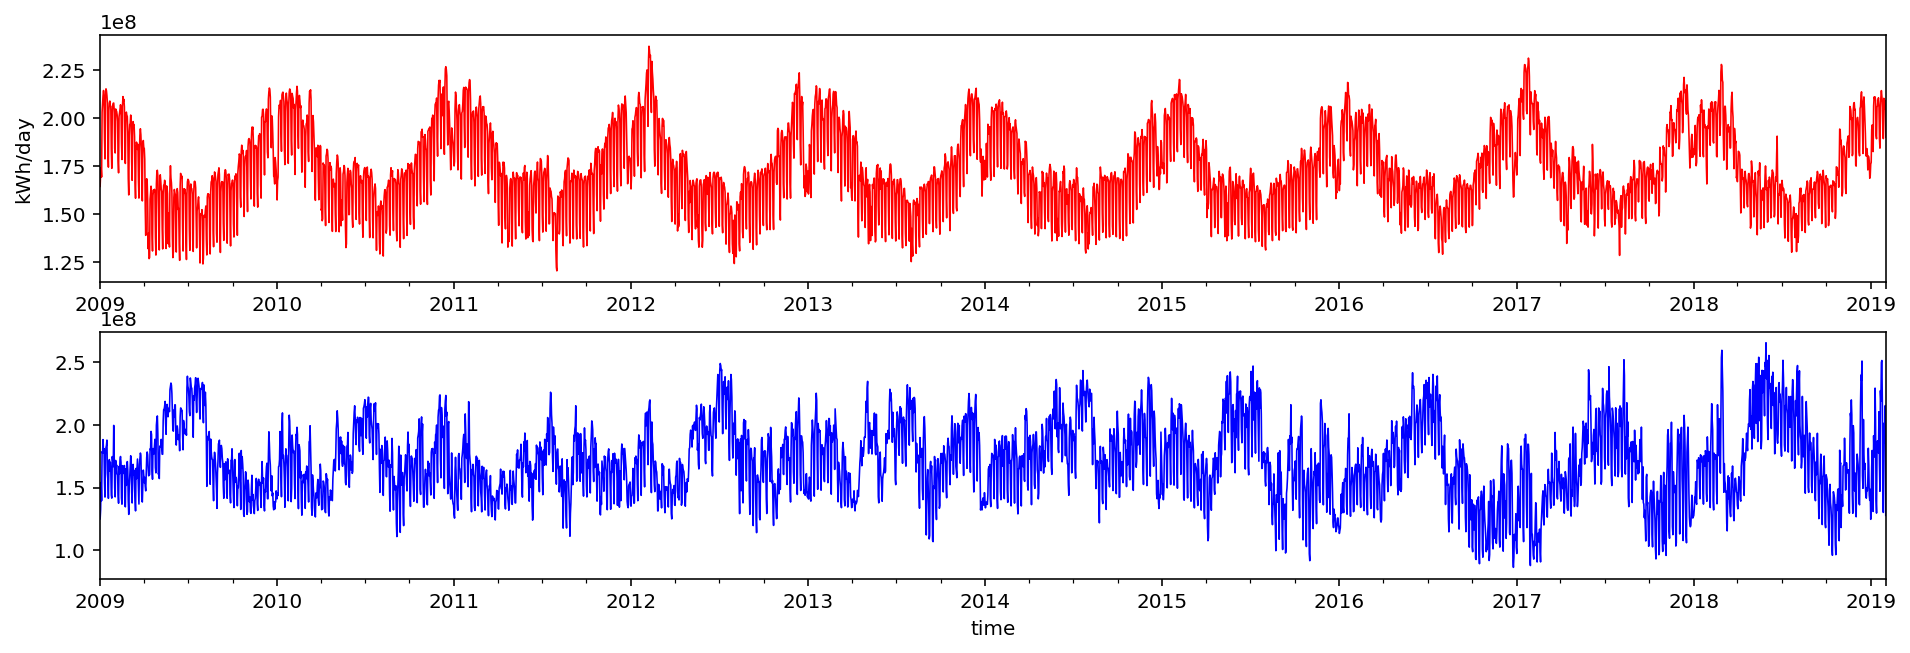
\includegraphics[width=\textwidth]{total_info.png}
    \caption{Daily energy consumption and production in Switzerland}
    \label{full dataset}
\end{figure}

\begin{figure}
    \centering
    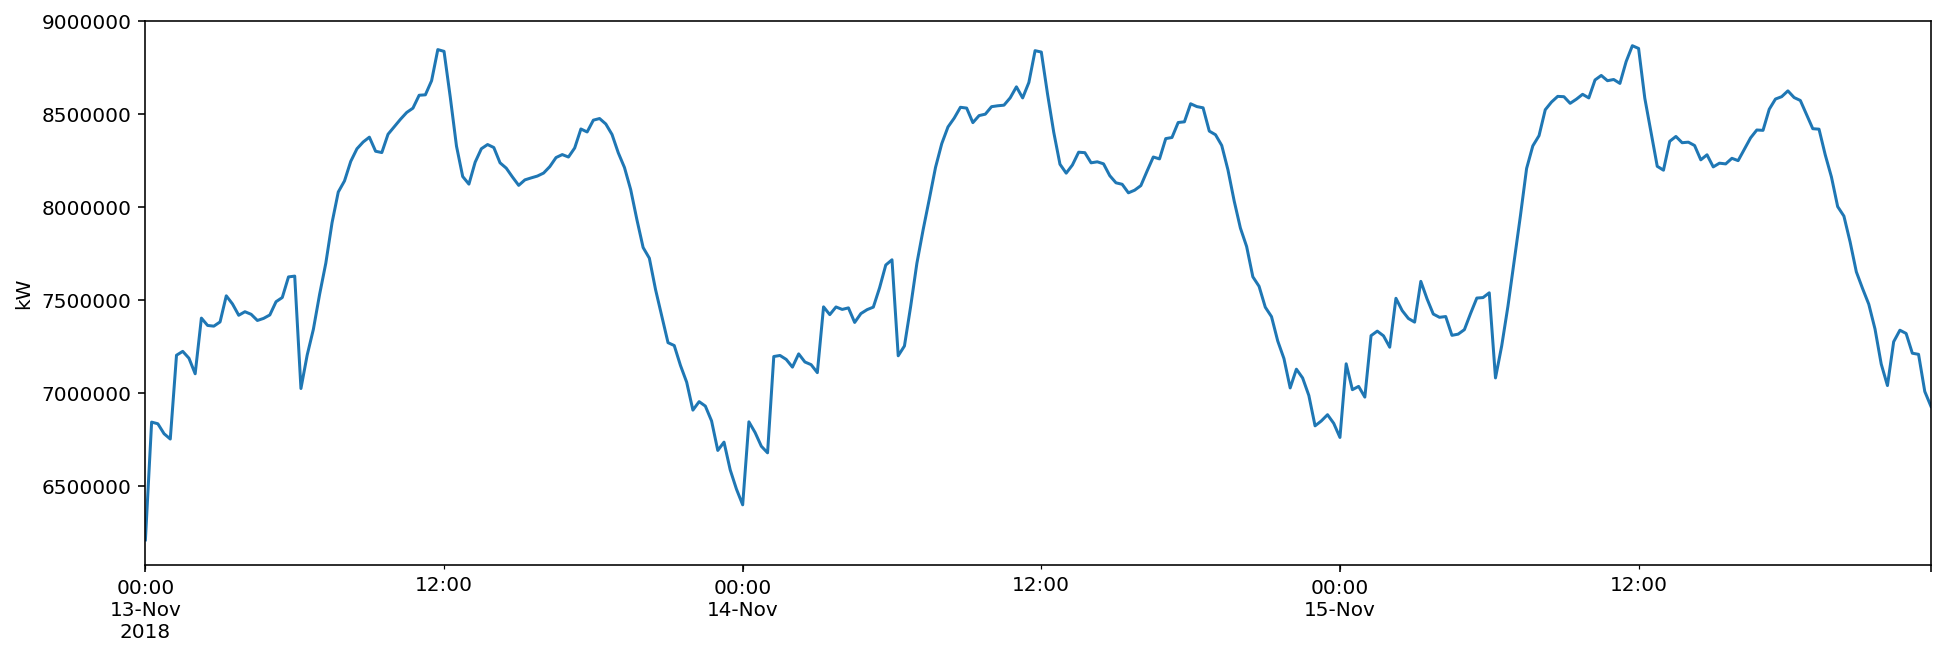
\includegraphics[width=\textwidth]{daily_seasonality.png}
    \caption{3 days of power consumption}
    \label{daily}
\end{figure}
\begin{figure}
    \centering
    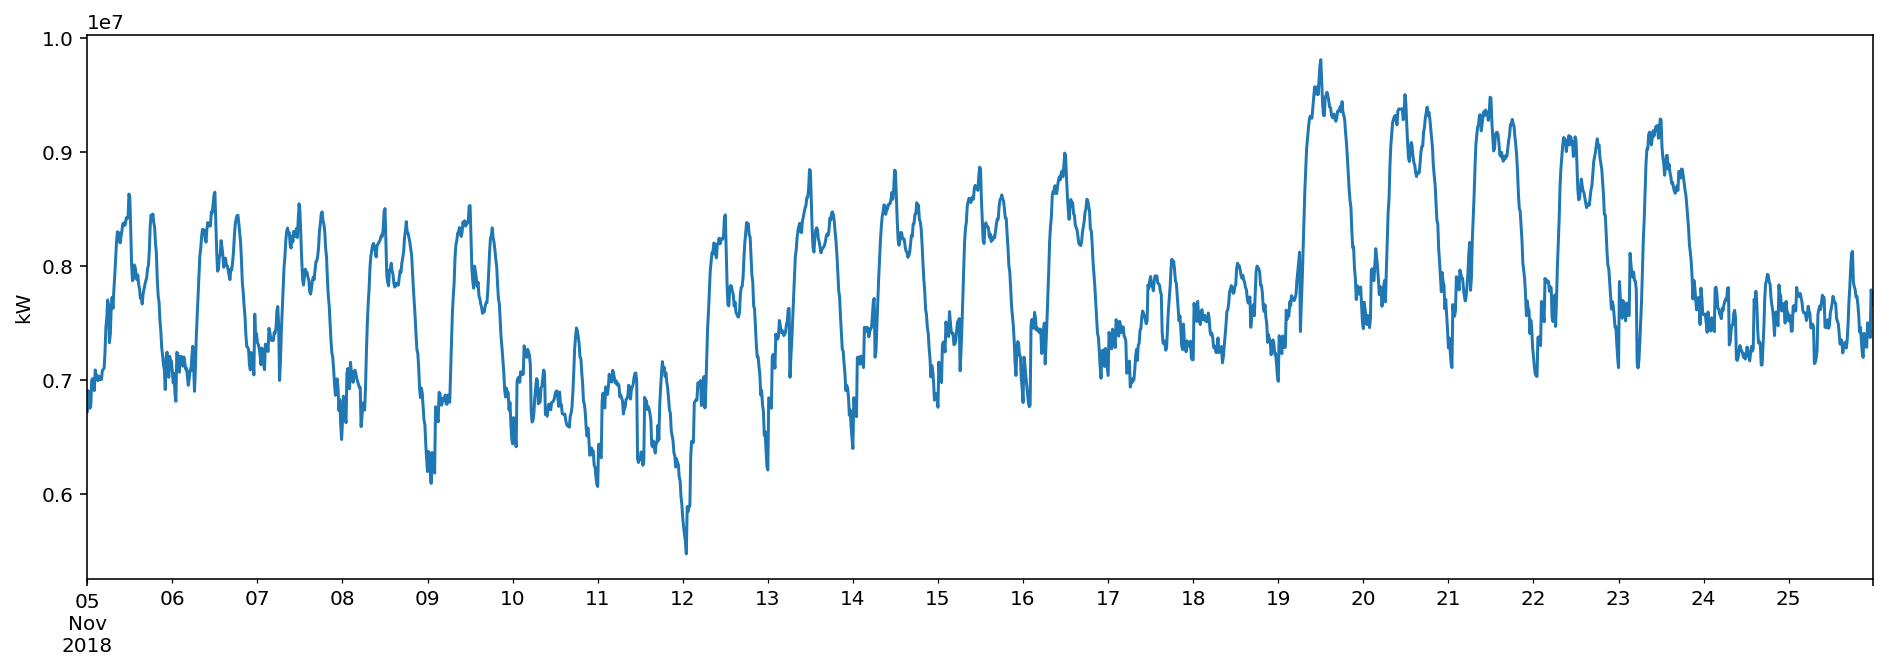
\includegraphics[width=\textwidth]{weekly_seasonality.png}
    \caption{3 weeks of power consumption}
    \label{weekly}
\end{figure}

\section{Aims and approach}
We anticipate that a big part of the work will deal with modeling the seasonal effects. Some of them have a precise periodicity, such as the 24 hours day cycle or the 7 day weekly ccycle, some other seasonal effects will require more attention: the exact date of the drop corresponding to easter holidays changes from year to year, and even festivities which happen at a fixed date, such as christmas, do not repeat at a completely regular pace, since some years count more days than others. A possible approach could be to introduce exogenous variables to represent holidays. We could eventually expand the model to account for the influence of weather variations on electrical demand.
Our final goal is to design a forecasting method for the consumption which could allow a controller of the power production facilities to minimize the difference between consumption and production.
As shown in figure \ref{rel_dif} at the moment the relative difference between the 2 quantities reaches some peaks of almost $80\%$. This might be a waste of money for the Swiss energy users, and also a damage for the environment since imported energy often comes from coal burning Germany.
Eventually, it could also be interesting to analyse the cantonal production/consumption in such a way to highlight how production could be tuned to minimize the losses due to energy transport between cantons.

\begin{figure}
    \centering
    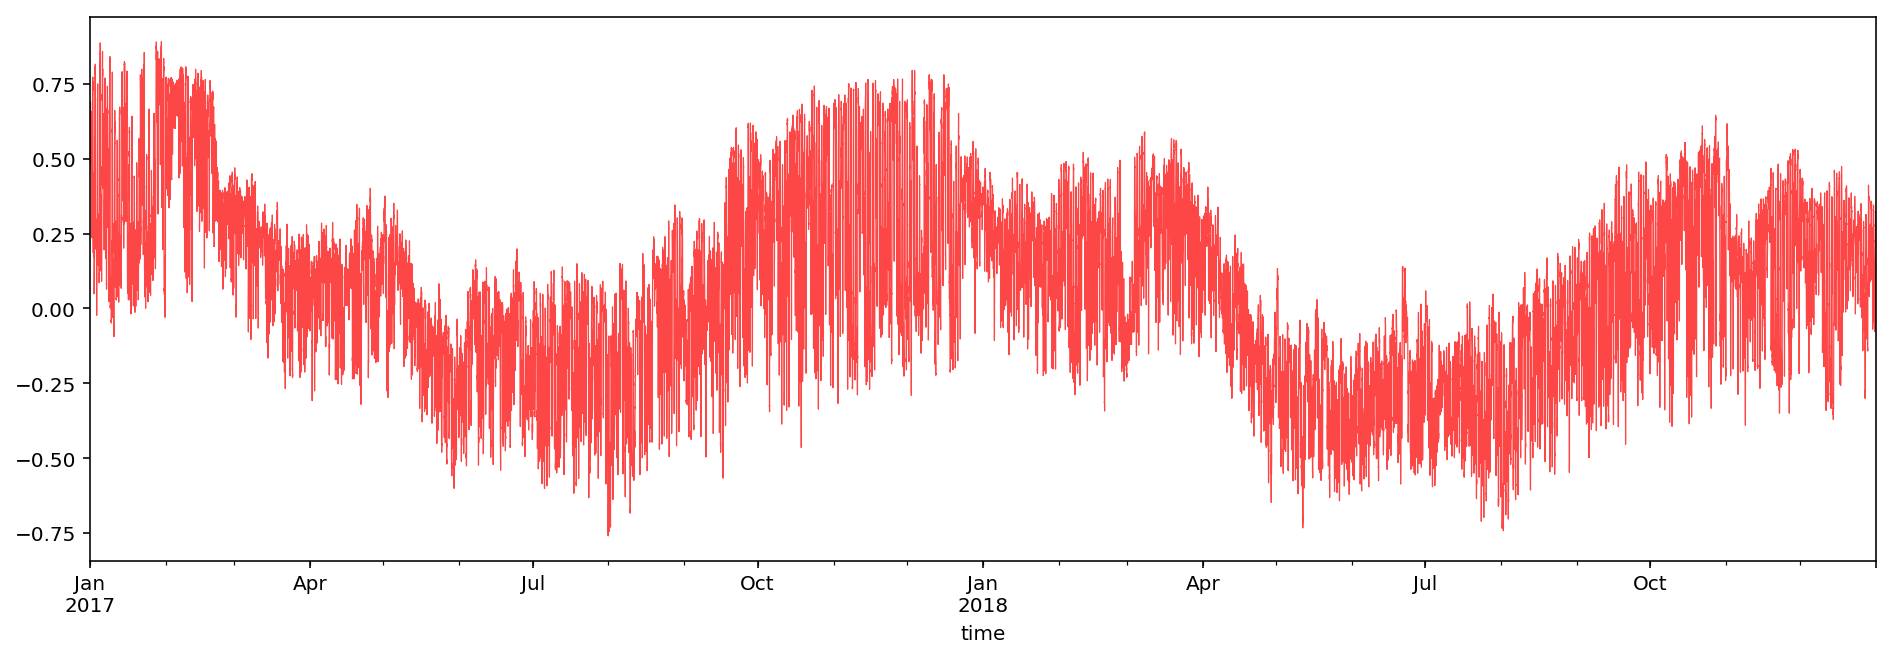
\includegraphics[width=\textwidth]{relative_difference.png}
    \caption{Relative difference between energy production and consumption computed as $d(a,b) = 2\frac{a-b}{a+b}$}
    \label{rel_dif}
\end{figure}
\section{Time Series Analysis}
% TODO add the description and comment to the classical threatment of the time series

\section{Multiple equation Time Series}
In this section we will propose a different method for the time series forecasting. In particular we will gradually create a multi equation model for the energy consumption forecasting. This paragraph is mainly focus on the work of \cite{quteprints95170}.
\subsection{A prototype model}
As seen in the previous paragraphs the energy consumption shows both a daily and weekly seasonality. So, it seems reasonable to start our model construction from an ARMA structure of the form
\begin{equation*}
L_h_d = \theta_{h0} + \theta_{h1}L_{h d-1} + \theta_{h2}L_{h d-7} + \phi_{h1]\varepsilon_{h d-1} + \psi_{h2}\varepsilon_{h d-7} + \varepsilon_{hd},
\end{equation*}
where L_{hd} is the load at time h of day d and $\varepsilon_{hd}$ is the disturbance term. Since we are using a half-hourly(?) sampled time series the index $h$ goes from $1$ to $48$. This kind of model reflects the idea that the energy load is correlated with the loads at the same half-hour in both the previous day and week.\\
The first important factor we have to add to the model is the public holiday information. In fact, the energy consumption is obviously infuenced by vacations. In order to economize on the number of parameters the vacation days are categorized in 6 groups: 4 unique special days (Good Friday, Easter Monday, Christmas day and New Years) and 2 switzerland bank holidays (1st of August and 20th September).\\ % TODO check if it true with Pietro
It is obvious that temperature must be taken into account too. The effect of high and low temperature must be threated in different ways and with this purpose the paper authors proposed the following piecewise linear specification:
\begin{equation*}
\mathbb{C}_{1hd} = 
\begin{cases}
0, & T_{hd}\leq 22\\
T_{hd} - 22, & 22 < T_{hd} \leq 30\\
30 - 22, & 30 < T_{hd} 
\end{cases}
\end{equation*} 
\begin{equation*}
\mathbb{C}_{2hd} = 
\begin{cases}
0, & T_{hd}\leq 26\\
T_{hd} - 26, & 26 < T_{hd} \leq 30\\
30 - 26, & 30 < T_{hd}
\end{cases}
\end{equation*}   
for the cooling degree temperature ranges and 
\begin{equation*}
\mathbb{H}_{1hd} = 
\begin{cases}
0, & 15 \leq T_{hd}\\
15 - T_{hd}, & 9 \leq T_{hd} < 15\\
15 - 9, & T_{hd} < 9
\end{cases}
\end{equation*}
\begin{equation*}
\mathbb{H}_{2hd} =
\begin{cases}
0, & 20 \leq T_{hd}\\
20 - T_{hd}, & 9 \leq T_{hd} < 20\\
20 - 9, & T_{hd} < 9
\end{cases}
\end{equation*} 
%probably we should change the temperature range since we are in switzerland and not in Australia
for the heating temperature ranges.\\
Incorporating these modifications into our model we obtain
\begin{gather}
L_h_d = \theta_{h0} + \theta_{h1}L_{h d-1} + \theta_{h2}L_{h d-7} + \phi_{h1]\varepsilon_{h d-1} + \psi_{h2}\varepsilon_{h d-7} + 
f^S_{hd} + f^T_{hd} + \varepsilon_{hd}\\
f^S_{hd} = \sum_{j=1}^6 \left(\alpha_{jh1}\mathbb{S}_{jhd} + \alpha_{jh2}\mathbb{S}_{jhd-1}\right)\\
f^T_{hd} = \sum_{k=1}^2\left\beta_{kh1}\mathbb{H}_{khd} + \beta_{kh2}\mathbb{C}_{khd} + \beta_{kh3}\mathbb{H}_{khd-1} + \beta_{kh4}\mathbb{C}_{khd-1} \right),
\end{gather}
where $f^S_{hd}$ and $f^T_{hd}$ are the special day and temperature effect respectively, $\mathbb{S}_jhd$ is the jth type of special day at half-hour interval h of day d.
\subsection{Extentions to the prototype model}

%-------------------------------------------------------------------------------
% REFERENCES
%-------------------------------------------------------------------------------
% \newpage
% \section*{References}

\bibliography{mybib} 
\bibliographystyle{ieeetr}



%[2]John W. Eaton, David Bateman, Sren Hauberg, Rik Wehbring (2015). GNU
%Octave version 4.0.0 manual: a high-level interactive language for numer-
%ical computations. Available: http://www.gnu.org/software/octave/doc/
%interpreter/. 
}
\end{document}

